\documentclass[tikz,border=2pt]{standalone}
\usepackage{amsmath}
\usetikzlibrary{arrows.meta}
\begin{document}
% Two routes to the cumulative sums of x = 1:6: a for loop filling a pre-allocated z in six
% passes, or one call cumsum(x). Both give 1, 3, 6, 10, 15, 21.
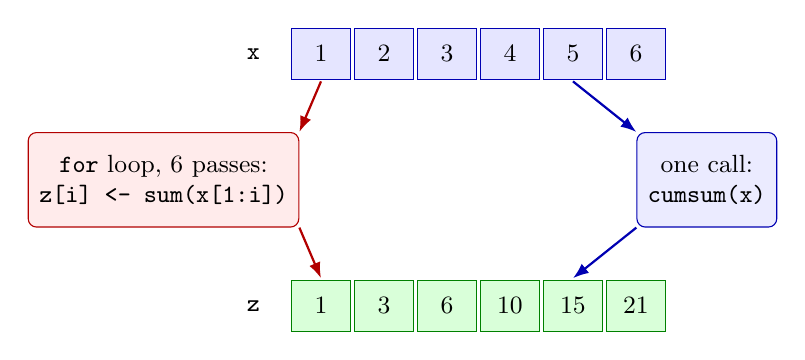
\begin{tikzpicture}[font=\small, >={Latex[length=2mm]},
  cell/.style={draw, minimum width=7.5mm, minimum height=6.5mm},
  box/.style={draw, rounded corners=3pt, align=center, inner sep=4pt, minimum height=12mm}]
  \node[anchor=east] at (2.35,0) {\texttt{x}};
  \foreach \v [count=\k] in {1,2,3,4,5,6} {
    \node[cell, draw=blue!70!black, fill=blue!10] at (2.2+0.8*\k,0) {\v};
  }
  \node[anchor=east] at (2.35,-3.2) {\texttt{z}};
  \foreach \v [count=\k] in {1,3,6,10,15,21} {
    \node[cell, draw=green!50!black, fill=green!15] at (2.2+0.8*\k,-3.2) {\v};
  }
  \node[box, draw=red!70!black, fill=red!8] (L) at (1.0,-1.6)
     {\texttt{for} loop, 6 passes:\\ \texttt{z[i] <- sum(x[1:i])}};
  \node[box, draw=blue!70!black, fill=blue!8] (R) at (7.9,-1.6)
     {one call:\\ \texttt{cumsum(x)}};
  \draw[->, thick, red!70!black] (3.0,-0.35) -- (L.north east);
  \draw[->, thick, red!70!black] (L.south east) -- (3.0,-2.85);
  \draw[->, thick, blue!70!black] (6.2,-0.35) -- (R.north west);
  \draw[->, thick, blue!70!black] (R.south west) -- (6.2,-2.85);
\end{tikzpicture}
\end{document}
